
The performance of \seidr{} is evaluated from several angles.
On classification, we are interested in the accuracy of \gls{acr:cca} detection using \gls{acr:iat} histograms, the time taken to train a model, and the required time to classify a flow.
In the \emph{2-class} problem, we investigate whether it is possible to separate \gls{acr:tcp} \emph{BBR} from \emph{Cubic} using \gls{acr:iat} histograms as the input data, while in the \emph{4-class} problem we extend this to include \emph{Reno} and \emph{Vegas}.
I compare this work against \textcite{DBLP:conf/icccn/HagosEYK18} in this regard.
On deployment, I demonstrate the bandwidth and memory requirements imposed by \seidr{}.

% Evaluation ideas for the system:
% \begin{enumerate}
%     \item Dataplane calculation: how many histograms can we do reasonable, how much memory space it needs
%     \item Show data reduction rates with dataplane aggregation - this depends on windowing as well - 1 ms, 100 ms - just back of the envelope calculation with some visualization. Assuume: per-flow histograms, packet size of 1500B, 100Gbit/s worth of traffic. 
% \end{enumerate}{}


% Evaluation ideas for the classification use-case:
% \begin{enumerate}
%     \item CNN classifier accuracy
%     \item CNN vs KNN vs LSTM vs K-means [traning time vs performance scatterplot]
%     \item Timestamp accuracy - importance of nanosecond timing from the dataplane
% \end{enumerate}

\subsection{Datasets}\label{sec:seidr-datasets}
We examine synthetic flows modelling bulk data transfer at various speeds, generated using iPerf3~\parencite{iperf3}, and processed using custom P4 firmware for Netronome \gls{acr:nfp} SmartNICs.
Packet captures and \gls{acr:iat} streams are publicly available~\parencite{ht-imc-data,ht-imc-poster}.
% Inter-arrival time streams are extracted using custom P4 firmware installed on Netronome Agilio CX 2x40GbE SmartNICs.
% Histograms are generated at classification time from these streams to ensure consistent input data and results between classification techniques and individual trials.
For every pairwise interaction between \gls{acr:tcp} \emph{BBR}, \emph{Cubic}, \emph{Reno}, and \emph{Vegas}, we capture solo and multiplexed dynamics by running each flow for \qty{3}{\second}, with \qty{2}{\second} of overlap (\ie, the second flow begins at $t=$~\qty{1}{\second}).
I observed that the first flow always completes slow-start before multiplexing begins, and by construction we have several unimpeded captures for every flavour.
The number or volume of multiplexed flows isn't expected to substantially alter captured dynamics (\ie, 3 flows at \qty{300}{\mega\bit\per\second} and 2 flows at \qty{200}{\mega\bit\per\second} should both have flows fall to \qty{100}{\mega\bit\per\second}).
Flows in one capture are generated using the same target rate in \{\num{100}, \num{200}, \dots, \num{1000}\} \unit{\mega\bit\per\second}, each uniformly randomly perturbed within $\pm$\qty{10}{\percent}.
We also control how this rate limit is applied: \emph{wire-limited} traffic uses \texttt{tc} in the Linux kernel to apply rate-limiting, while \emph{application-limited} traffic uses iPerf's built-in mechanisms to control send rate.
Application-limited traffic leads to specific behaviour in \emph{BBR} and some other flavours, while wire-limited traffic creates loss events as the rate grows too high (which can expose additional behaviours in response to such events).
\num{10} such captures are recorded for each $\left(\mathit{CCA}_1,\mathit{CCA}_2,\mathit{speed},\mathit{limiter}\right)$ tuple, and generated flows are labelled accordingly.

\gls{acr:iat} streams are broken down into overlapping sequences of the required length, before being histogrammed as required into \num{100} buckets over \qtyrange{0}{1}{\milli\second}.
The use of overlapping sequences extends the training and testing sets significantly, while ensuring that larger sequences don't result in a far smaller training corpus.
Cross-validation occurs on a per-flow basis rather than per-sequence, \ie, sequences from the same flow must only appear in \emph{either} the test or training set.
This ensures stringent data hygiene, and prevents adjacent sequences from inducing overfitting.
All classifier evaluation which follows uses 4-fold cross-validation.
The data is comprised of \num{4994} flows (\num{832} in \emph{2-class}), or \numrange{18}{31} million sequences (\numrange{3.2}{5.2} million in \emph{2-class}).

\subsection{Experimental setup}
All experiments were executed on a single machine running Ubuntu 18.04.4 LTS (GNU/Linux 4.15.0-96-generic x86\_64), using an Intel Core i7-6700K \gls{acr:cpu} (\qtyproduct[product-units=single]{4 x 4.2}{\giga\hertz}) which had \SI{32}{\gibi\byte} of \gls{acr:ram}.
\gls{acr:cnn} training was performed using Nvidia RTX 2080Ti cards (\qty{11}{\giga\byte} GDDR6 \gls{acr:vram}).
For the dataplane, we used multiple Netronome Agilio CX \numproduct{2 x 40}GbE SmartNICs using \qty{40}{\giga\bit\per\second} connections between source and destination hosts.
% All code underpinning these findings is available on a public
% repository

% All our experiments are run on ESnet's test setup, using production servers with Intel Xeon Gold 6242 CPUs clocked at \SIrange{2.8}{3.9}{\giga\hertz} (32 cores) and \SI{793}{\giga\byte} of RAM.

\subsection{Classification performance}
In the \emph{2-class} formulation, we can observe from \cref{fig:2c-results} that \gls{acr:cnn} performance increases slightly with the length of the input sequence for classifying application-limited traffic.
\gls{acr:cnn}-based detection has a peak F1-score of \num{0.965} for application-limited traffic, and \num{0.894} when wire-limited.
This increase does not extend towards histograms taken over the entirety of each flow (\emph{Full}), which are hampered by having 6 orders of magnitude fewer training samples.
While very effective, \glspl{acr:knn} come with significant memory cost.
By design, the entire dataset must be kept in memory: for subflow histograms of length \num{500} packets, this equates to \qty{1.5}{\gibi\byte} of training data.
Naturally, this is undesirable for many network deployments, where easy relocation of inference may be key.

\begin{figure}
    \centering
    \resizebox{\linewidth}{!}{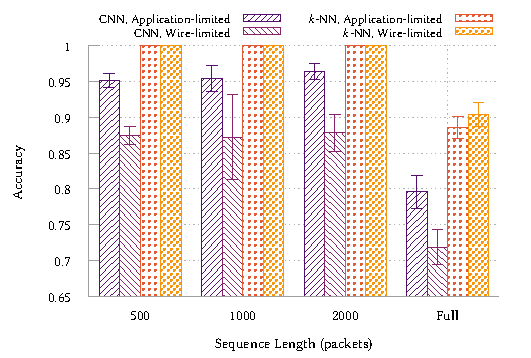
\includegraphics{plots/seidr/2class-results-thesis.pdf}}
    \caption[Accuracy of $k$NN and CNN classifiers when classifying \emph{BBR} and \emph{Cubic} TCP traffic from IAT histograms, trained  over various sequence lengths.]{
    	Accuracy of \gls{acr:knn} and \gls{acr:cnn} classifiers when classifying \emph{BBR} and \emph{Cubic} \gls{acr:tcp} traffic from \gls{acr:iat} histograms, trained over various sequence lengths.
    	In both subsequences and complete flow histograms, accuracies are generally high (at least \qtylist{87; 72}{\percent} respectively).
    	\glspl{acr:knn} outperform the \gls{acr:cnn} architecture here, otherwise we generally see that longer subsequences offer some improvement to application-limited accuracy, and wire-limited \emph{Cubic} and \emph{BBR} are harder to tell apart.
 		\label{fig:2c-results}
    }
\end{figure}

\begin{figure}
    \centering
    \resizebox{\linewidth}{!}{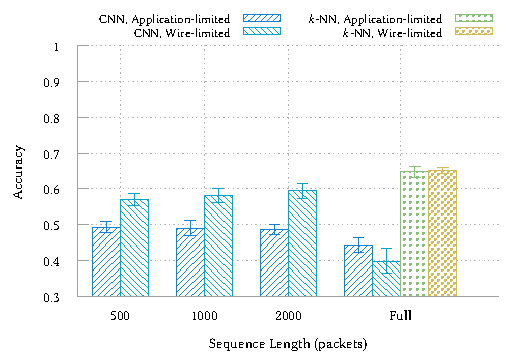
\includegraphics{plots/seidr/4class-results-thesis.pdf}}
    \caption[Accuracy of $k$NN and CNN classifiers when classifying \emph{BBR}, \emph{Cubic}, \emph{Reno}, and \emph{Vegas} TCP traffic from IAT histograms, trained and tested on various sequence lengths.]{
    	Accuracy of \gls{acr:knn} and \gls{acr:cnn} classifiers when classifying \emph{BBR}, \emph{Cubic}, \emph{Reno}, and \emph{Vegas} \gls{acr:tcp} traffic from \gls{acr:iat} histograms, trained and tested on various sequence lengths.
    	\glspl{acr:knn} again achieve better performance here, but when handling subflows the entire corpus cannot fit into \gls{acr:ram}.
    	We see instead that wire-limited traffic is easier to classify when all 4 \glspl{acr:cca} are examined: again, this performance increases with histogram sequence length.
    	\label{fig:4c-results}
    }
\end{figure}

\Cref{fig:4c-results} shows in the \emph{4-class} case that we observe a sharp loss in classification accuracy, peaking at \qty[uncertainty-mode=separate]{59.5 +- 2}{\percent} for \glspl{acr:cnn} and \qty[uncertainty-mode=separate]{64.5 +- 1.6}{\percent} for \glspl{acr:knn}.
This suggests that \gls{acr:iat} histograms don't generalise as an effective feature for other \gls{acr:tcp} flavours.
Exploratory work with \glspl{acr:lstm} on \gls{acr:iat} streams confirmed that this persists before aggregation.
Likewise, exclusive pairwise training did not lead to an increase in accuracy.
However, \cref{fig:4c-cnn-conf} shows that timing information remains key in separating BBR from its predecessors to a high degree of accuracy, confirming our hypothesis that its \emph{timer}-based (rather than \texttt{cwnd}-based) design allows for this detection.
If this marker were present between \emph{loss}- and \emph{delay}-based variants, then we'd also see high predictive power over \emph{Vegas} traffic.
Breaking down these confusion matrices by rate limit type sheds still more light.
In \cref{fig:4c-cnn-conf-app}, application-limited data transfers are almost indistinguishable using these metrics (aside from \emph{Vegas}), while \cref{fig:4c-cnn-conf-tc} reveals that \glspl{acr:iat} hold some discriminative power for wire-limited Cubic traffic.
Note that \emph{4-class} \gls{acr:knn} experiments on all but full sequences required excessive memory and classification time, and so are excluded.
While full-sequence \glspl{acr:knn} outperform all examined \glspl{acr:cnn} on this task (respective peak F1-scores \num{0.697} vs.\@ \num{0.486}), these reduce $\mathit{F1}_\mathit{BBR}$ from \num{0.935} to \num{0.810}.

\begin{figure}
    \centering
    \begin{subfigure}[b]{\linewidth}
    \centering
    \resizebox{1.0\linewidth}{!}{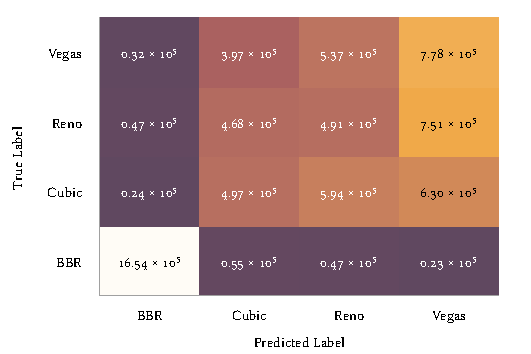
\includegraphics{plots/seidr/cnn-histo-app-confusion-2000-thesis.pdf}}
    \subcaption{\emph{Application-limited}. $\mathit{F1}_\mathit{BBR}=$~\num{0.935}, $\mathit{F1}=$~\num{0.486}.
    \label{fig:4c-cnn-conf-app}
    }
    \end{subfigure}%

    \begin{subfigure}[b]{\linewidth}
    \centering
    \resizebox{1.0\linewidth}{!}{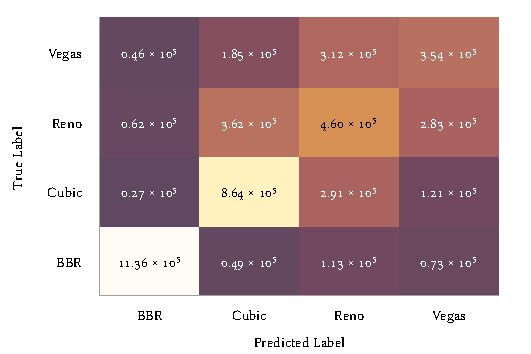
\includegraphics{plots/seidr/cnn-histo-tc-confusion-2000-thesis.pdf}}
    \caption{\emph{Wire-limited}. $\mathit{F1}_\mathit{BBR}=$~\num{0.893}, $\mathit{F1}=$~\num{0.573}. 
    Notably, $\mathit{F1}_\mathit{Cubic}=$~\num{0.625}.
    \label{fig:4c-cnn-conf-tc}
    }
    \end{subfigure}
    
    \caption[Confusion matrices for a CNN on the \emph{4-class} problem, \num{2000}-packet length sequences.]{Confusion matrices for a \gls{acr:cnn} on the \emph{4-class} problem, \num{2000}-packet length sequences. Brighter entries along the diagonal indicate correct classifications. BBR remains easy to distinguish regardless of the rate limit mechanism, while Cubic is slightly more distinct from its \texttt{cwnd}-based alternatives for wire-limited traffic. \glspl{acr:cca} are generally easy to tell apart in wire-limited traffic---this is sensible, in that most \gls{acr:cca} differences will arise in response to congestion events rather than application behaviour, and matches the general trends seen in \cref{fig:4c-results}.}
    \label{fig:4c-cnn-conf}
\end{figure}

I contrast this work with that of \textcite{DBLP:conf/icccn/HagosEYK18}, who employ \glspl{acr:cnn} to predict \texttt{cwnd} size for any flow from its stream of bytes-in-flight measurements.
On detection of a loss event the \emph{multiplicative decrease} $\beta$ is measured from estimated \texttt{cwnd}s, from which the \gls{acr:cca} may be classified.
In identifying \gls{acr:tcp} \emph{BIC}, \emph{Cubic}, and \emph{Reno}, they achieve \qty{95}{\percent} accuracy, which outperforms \seidr{} on \texttt{cwnd}-based \glspl{acr:cca}.
% ??Their work aims to capture the dynamics of loss-based CCAs, but we claim that the shared factor is in fact the reliance upon a sliding congestion window.
Yet their approach cannot work for detecting \emph{BBR}. 
\emph{BBR} is not based upon the notion of a sliding congestion window, so there is no parameter $\beta$ to infer.
Although \gls{acr:iat} histograms are suitable for \emph{BBR} detection due to the intrinsic properties of its algorithm, we envision that this approach could be augmented by using a negative \emph{BBR} classification to trigger \texttt{cwnd} estimation.
Having seen that some predictive power from \glspl{acr:iat} is preserved for \texttt{cwnd}-based \glspl{acr:cca}, we expect that this will increase the accuracy of a universal classifier.
It is important, however, that this step be taken adaptively; this incurs higher resource requirements for bytes-in-flight tracking and for efficient handling of potential return-path asymmetry.
\seidr{} on its own does not add such overheads or operational complexity, and does not require a telemetry system to see or detect \texttt{cwnd} adjustments by the sender.

\subsection{Training and inference costs}
\begin{table}[]
    \centering
    \caption[Training, inference, and runtime memory costs of CNN and $k$NN models.]{Training, inference, and runtime memory costs of \gls{acr:cnn} and \gls{acr:knn} models.}
%    \resizebox{0.8\linewidth}{!}{
    \expandableinput{tables/seidr/train-times}
%	}
    \label{tab:train-test-times}
\end{table}

Typical test and training times for these \gls{acr:ml} classifiers and problem formulations are lsited in \cref{tab:train-test-times}.
Training times for \glspl{acr:knn} include the time taken to load and process the entire training set, and are incurred \emph{every time} the model is started on a new host.
\glspl{acr:cnn} trained for online analysis (flow subsequences) achieve the lowest per-flow inference times, and are increased during offline analysis due to worse batching and cache behaviour on the smaller data set.
While \glspl{acr:knn} are effective in many cases, I find they are only computationally viable when offline (\ie, full-flow histograms), as the entire test data corpus must remain in memory.
A single \emph{4-class} cross-validation fold (\num{2000} packets) required 3 days to train and test over the entire dataset, which was deemed to be outright infeasible.
In contrast while online \glspl{acr:cnn} take longer to train, they have a considerably lower memory footprint, the training cost is paid only once, and flows may be classified in real-time with milliseconds of total observations.

\subsection{Switch resource usage}
The implementation of \seidr{} requires an extra table in the ingress pipeline to update buckets, update configuration, and rewrite packets.
If digests are used rather then clone-based packet rewriting, then this table may be placed in either ingress or egress.
Further code space is required to include a configuration packet parser.
Shared configuration data (registers \numrange{1}{5}) requires \qty{42}{\byte} per switch, while each flow requires \qtylist{224;248}{\byte} to store buckets, counters, previous timestamps, and active 5-tuples on IPv4/v6 networks respectively.
On platforms which support hash-table structures, this cost scales linearly with the number of tracked flows.
Otherwise, this requires pre-allocation of an entry for every possible hash value (\eg, \qtyrange{14}{15.5}{\mebi\byte} for a \qty{16}{\bit} hash). This small memory requirement fits histogram generation to all devices available today.

\subsection{Quantifying in-network data aggregation}

\begin{figure}
    \centering
    \resizebox{1\linewidth}{!}{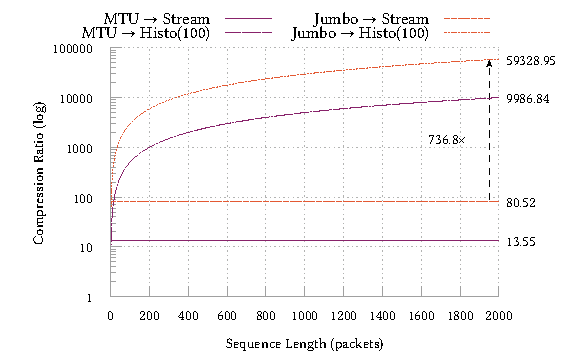
\includegraphics[trim=14 0 0 0,clip,width=\textwidth]{plots/seidr/compression-v6-thesis.pdf}}
    \caption[Compression ratio of \num{100}-bucket histograms and timestamp streams from raw packets on an IPv6 network.]{Compression ratio of \num{100}-bucket histograms and timestamp streams from raw packets on an IPv6 network. As sequence length increases, histograms provide more of an advantage in compression rate, being \qty{736.8}{\times} smaller than timestamp streams when analysing \num{2000}-packet sequences.}
    \label{fig:histo-compression}
\end{figure}

% \begin{figure}
%     \centering
%     \resizebox{\linewidth}{!}{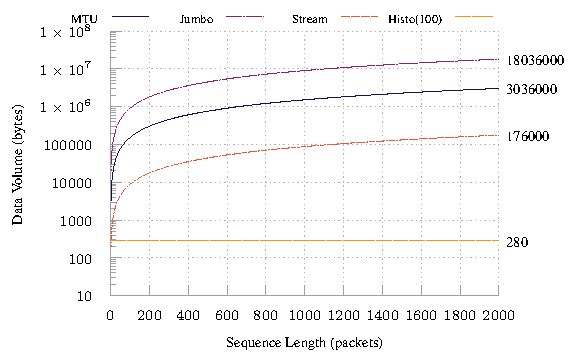
\includegraphics{plots/seidr/histo-sz-v6.pdf}}
%     \caption{Data volume of 100-bucket histograms and timestamp streams versus raw packets on an IPv6 network.}
%     \label{fig:histo-sz}
% \end{figure}
To show data rate reductions, I compute the compression ratio of generated histograms against various other representations which can be used to move \glspl{acr:iat} (or the packets used to compute them) from the dataplane.
Although it is more commonly a metric used for compression algorithms, it is simply:
$$\mathit{Compression Ratio} = \frac{\mathit{Uncompressed Size}}{\mathit{Compressed Size}}$$
\Cref{fig:histo-compression} demonstrates the reduction in data sent from raw mirrored packets, to a stream of measured timestamps or \glspl{acr:iat}, to \seidr{} histograms on an IPv6 network.
Timing histograms naturally provide a larger data reduction as the amount of measured packets increases, while a per-packet \gls{acr:iat} or telemetry stream offers no reduction in packet rate.
Due to this, 100-bucket histograms cause a greater data reduction than per-packet \glspl{acr:iat} after just 4 packets in a sequence, and consume \qty{736.8}{\times} less volume for \num{2000}-packet sequences.

To make this concrete, \qty{100}{\giga\bit\per\second} traffic is reduced to \qty{10.01}{\mega\bit\per\second} additional switch traffic for \gls{acr:mtu}-size packets, and to \qty{1.69}{\mega\bit\per\second} for jumbo frames.
\gls{acr:iat} streams, by comparison, reduce to \qty{7.38}{\giga\bit\per\second} (resp.\ \qty{1.24}{\giga\bit\per\second}).
For a flow at \qty{100}{\mega\bit\per\second}, only \qty{30}{\milli\second} is needed to collect enough packets to make a classification.
Scaling beyond this, packet processing rates are the bottleneck.
As commodity machines and today's stream processors have a reasonable upper bound of $\sim$\qty[per-symbol=p,sticky-per=true]{1}{\mega\packet\per\second} processing capacity~\parencite{DBLP:conf/sigcomm/GuptaHCFRW18}, \seidr{} could scale up to \qty{1}{\tera\bit\per\second} \gls{acr:mtu}-size packet traffic on one machine, which would correspond to only \qty[per-symbol=p,sticky-per=true]{333}{\kilo\packet\per\second} histogram packets (\qty[per-symbol=p,sticky-per=true]{55.6}{\kilo\packet\per\second} if jumbo-size).
Reliably scaling to \qty{10}{\tera\bit\per\second} and beyond requires only that we increase the histogram sequence length to $\ge$\num{7000} packets.

